\chapter{Реализация программного продукта}

В этой главе описаны практические методы и их частичное представлении реализации, 
которые мы использовали для достижения поставленной цели.

\section{Использование парсера данных}

Так как для обучения нейронной сети статическим контентом, а именно: сайты с анекдотами и сайты со сценариями юмористических сценок. 
Для того чтобы собрать все эти данные потребуется решить задачу парсинга нужны большие массивы данных, возникает задача сбора данных 
относящихся к юмору(тории юмора). Источников таких данных не так много, основынми будут веб ресуры с юморивеб сайтов.

Поэтому опишем алгоритм решающий такую задачу. В качестве вводных возьмем url ссылки на веб ресурсы. 
Так как веб сайты могут иметь разную архитектуру возникает задача построения унификационного решения данного вопроса.

Как было описано ранее для полного парсинга страницы необходимо использовать рекурсивный метод, принцип которого подробно описан в parser02, 
который выражен в том, что мы проходим все ссылки на выбранном ресурсе. Основная функциональность заключается в следующих строчках :

\begin{figure}[H]
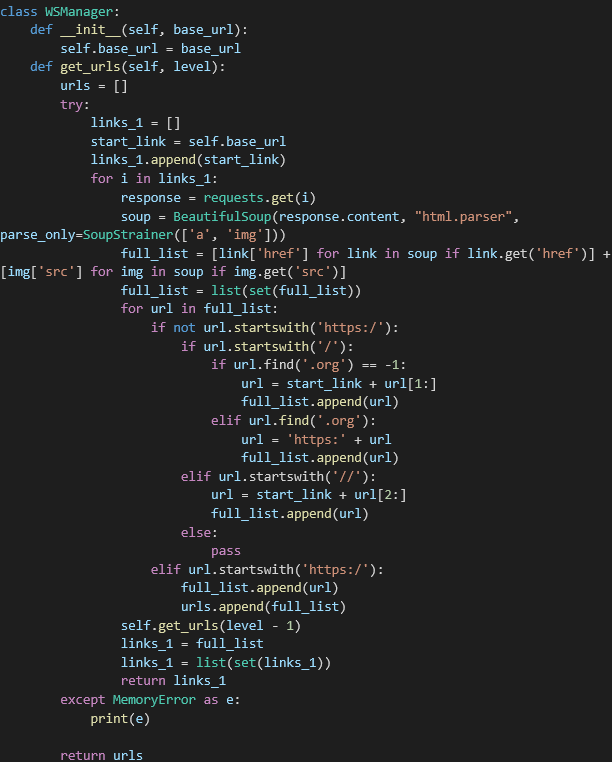
\includegraphics[width=0.75\columnwidth]{./img/code_block_1.png}
\centering
\caption{Класс WSManager - Основная функциональность рекурсивного парсинга}
\label{pic:code_block_1.png}
\end{figure}

Имея ссылку на страницу, мы можем полуть html код страницы. По выше указанному коду найдем все ссылки на ресурсы данного веб 
сервиса предоставленные на этой странице. Осмотрим все полученные ссылки таким же образом. В итоге мы получим html коды 
практически всех страницы доступных на принятом в рассмотрение ресурсе.

URL ссылки на веб сервисы предоставляющие, данные о юмористических текстах, агрегируются в экземплярах класса WSManager 
(Web Site Manager). Далее каждый экземпляр класса создает и запускает экземпляры класса RManager (Request Manager). 
Которые занимаются асинхронным получением данных с сайтов.    

Для классического получения данных при наличии API, код будет выглядеть следующим образом:

\begin{figure}[H]
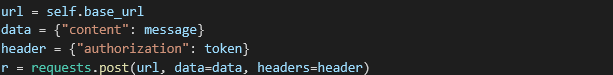
\includegraphics[width=0.75\columnwidth]{./img/code_block_2.png}
\centering
\caption{Получения данных при наличии API}
\label{pic:code_block_2.png}
\end{figure}

При получении положительного ответа 200, запрос отработал успешно.
В данной работе класс RManager использует корутины, что позволяет существенно сэкономить время ожидания всех ответов веб сервисов. 
Указанная экономия целиком и полностью объясняется тем, что пока класс ожидает ответ на первые запросы, он не перестает слать последующие. 
А те запросы, ответ на которые уже был получен, передаются в экземпляры класса  WHParser так, что на каждую полученную html страницу 
создается один экземпляр такого класса.

\begin{figure}[H]
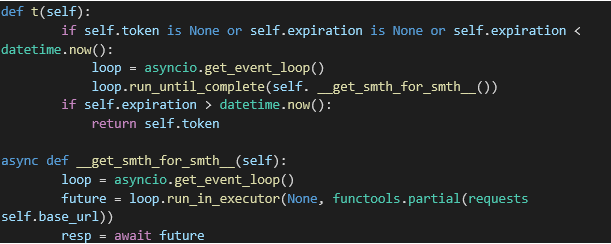
\includegraphics[width=0.75\columnwidth]{./img/code_block_3.png}
\centering
\caption{функция получения данных HTML класса WHParser}
\label{pic:code_block_3.png}
\end{figure}
  

Предположим, что на сайте еще стоит ограничение по запросам, поэтому предварительно, мы имеем лист проверенных и подготовленных рабочих прокси. 
При этом статусы готовности, которых получены в отдельных скриптах языка python3 с использованием корутин из программного модуля asyncio.

\begin{figure}[H]
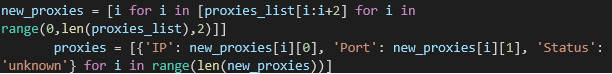
\includegraphics[width=0.75\columnwidth]{./img/code_block_4.png}
\centering
\caption{Обработка proxy}
\label{pic:code_block_4.png}
\end{figure}
    

\begin{figure}[H]
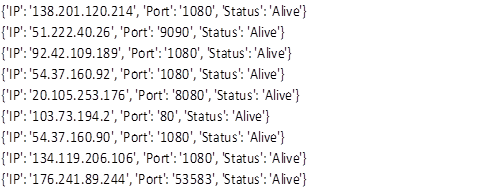
\includegraphics[width=0.75\columnwidth]{./img/ris13.png}
\centering
\caption{Проверка статуса прокси серверов}
\label{pic:ris13}
\end{figure}

Далее помещаем наши прокси в ассинхронные запросы так, что при неудовлетворительном ответе с сервера, 
класс RManager меняет используемую прокси.


\begin{figure}[H]
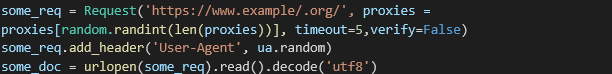
\includegraphics[width=0.75\columnwidth]{./img/code_block_5.png}
\centering
\caption{пример работы RManager}
\label{pic:code_block_5.png}
\end{figure}

WHParser, получив код веб страницы, обрабатывает его с помощью модуля BaeautifulSoup. 
Выделяет текста на основании тегов, определенных экспертами для каждого веб сервиса. 
soup = BeautifulSoup(some\_doc, 'html.parser')

Для вытаскивания данных из таблиц используем обращения к классам HTML. Атрибут class указывает одно или несколько классов для элемента. 
Атрибут class используется в основном для того, чтобы указывать на класс в таблице стилей. Однако он также может использоваться 
JavaScript (через HTML DOM) для внесения изменений в элементы HTML с указанным классом. Так же надо учесть то, что текстовые 
элементы традиционно заключают в элементы с теговым названием “p”, но полный семантически связанный текст может быть разбит 
множества предложений, таким образом, что отдельные элементы одного и того же уровня вложенности будут представлять эти разбитые множества. 
В связи с этим возникает задача восстановления семантически связанного текста из элементов одинаковой вложенности и одинакового типа, 
что следует учитывать при дальнейшей разработке.

\begin{figure}[H]
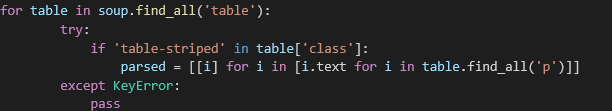
\includegraphics[width=0.75\columnwidth]{./img/code_block_6.png}
\centering
\caption{Обращение к атрибутам HTML}
\label{pic:code_block_6.png}
\end{figure}

Получаем данные в формате:

\begin{figure}[H]
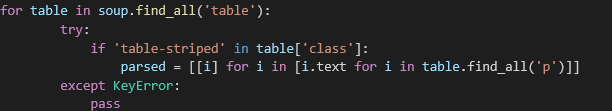
\includegraphics[width=0.75\columnwidth]{./img/code_block_6.png}
\centering
\caption{Полученные данные}
\label{pic:code_js.png}
\end{figure}


\section{Анализ и отбор полученных данных}

После получения текстовых данных с выбранных ресурсов, требуется провести просеивание массива на данные, 
излишне затронутые в процессе парсинга, так как на сайте слишком много текста и достаточно большой процент 
содержания лишнего текста по типу маркировок, контекстной рекламы и прочего, а наша задача получить интересующие 
нас юмористические текстовые данные в совокупности html страниц.

Значимый текст выбирается на основании анализа его принадлежности к заранее определенным классам текста (или тематикам). 
Как правило, методы автоматической классификации основаны на методе машинного обучения: сначала получают обученную с 
помощью какого-либо алгоритма модель, качество которой определяет точность классификации. Таким образом, процесс 
обучения зависит от выбранного алгоритма и «чистоты» обучающей выборки. Для решения такой проблемы выделим тэги и 
классы элементов, содержащих юмористические данные. Чтобы понять какие данные нам подходят, а какие нет. 

Следует учесть, что большое количество классов (десятки и сотни) приводит к увеличению трудоемкости обучения и 
понижению точности классификации, которая описана в \cite{neural06}. Тематики в юморе, близки по своей сути (например, экономика и бизнес), что 
приводит к тому, что классы в обучающей модели начинают пересекаться, приводя к снижению точности. 

В таких случаях, классификация проходит по принципу объединения классов в один, а затем используют под классификацию 
или повторную классификацию документов внутри класса.

В данной системе автоматической классификации используется популярный метод опорных векторов (или SVM – Support Vector Machine) 
с мерой TFiDF \cite{seman05}. Написано консольное приложение на языке программирования C\#, целью которого ставится использование библиотеки  
dll - LingvoNET, которая представляет собой модель специально обученную на нескольких классах, определенных заранее, 
принцип проектирования описан в \cite{neural09}. 
Для использования данного ресурса в проекте реализуется класс написанные на языке программирования Python, который 
взаимодействует с консольным приложением через стандартный вход и стандартный выход.

Классы содержащиеся в библиотеке LingvoNET – представлены ниже:
\begin{itemize}
  \item Экономика и бизнес
  \item Шоу-бизнес и развлечения
  \item Семья
  \item Мода
  \item Компьютерные игры
  \item Здоровье и медицина
  \item Политика
  \item Наука и технологи
  \item Спорт
  \item Туризм, путешествия
  \item Недвижимость
  \item Авто
\end{itemize}

Согласно этим классам, происходит классификация каждого входящего текста с учетом его меры близости к тому или иному классу, 
так же как и в юморе чаще всего есть семантическая принадлежность к тому или иному классу представленному выше, однако такие 
классы как “Игры”, “Спорт”, “Мода”, “Авто” и “Недвижимость”, чаще всего относятся к контекстной рекламе. 
Если документ близок к двум тематикам, то он попадает в соответствующие два класса. 
Если текст похож сразу на несколько тематик, то, скорее всего, это шум и не семантически не подходит.

Качество классификации чаще всего оценивается по двум критериям: точностью и полнотой классификации согласно работе \cite{neural07}.

Точность - показывает, насколько точно тексты с ресурсов попадают в определенный класс.

Полнота - определяется соотношением текстов, релевантных данному классу, к общему количеству релевантных текстов. Точность можно повышать, задавая порог прохода текста в тот или иной класс, при этом полнота классификации будет уменьшаться. Как правило, стараются найти оптимальное соотношение этих критериев.

Представим пример полученного текста с ресурса:

\begin{itemize} 
  \item Мам, помоги с сочинением. Нужно не меньше 350 слов.
  \item А что за тема? 
  \item Некрасов: "Кому на Руси жить хорошо". 
  \item Напиши — "депутатам".
  \item Но надо 350 слов.
  \item Пиши поименно!
\end{itemize}

В данном случае получим следующие результаты анализа представленных выше  данных:

\begin{table}[H]
  \caption{Результат семантического анализа подходящего текста}
  \label{tbl:text_a01}
  \begin{center}
  %\centering
  \begin{tabular}{ | c | c | }
    \hline
    Семья	& 46.81\% \\ \hline
    Политика &	19.17\% \\ \hline
    Другие	& менее 10\% \\ \hline
  \end{tabular}
  \end{center}
\end{table}

Текст будет отнесен к классу “Семья” и семантически подходит нам в качестве искомого вида юмористического текста.
	
Иной же случай, это пример контекстной рекламы:
“Горячие предложения контрафактного алкоголя на каждой подворотне! Тема, которая волнует репортерское агентство в этом городе. Бодяжная сивуха убивает людей, о чем думает администрация???”

\begin{table}[H]
  \caption{Результат семантического анализа не подходящего текста}
  \label{tbl:text_a02}
  \begin{center}
  %\centering
  \begin{tabular}{ | c | c | }
    \hline
    Недвижимость &	14.18\% \\ \hline
    Здоровье и медицина	& 12.25\% \\ \hline
    Политика & 11.55\% \\ \hline
    Семья	& 10.91\% \\ \hline
    Экономика и бизнес & 10.45\% \\ \hline
    Шоу-бизнес и развлечения & 10.02\% \\ \hline
    Другие & менее 10\% \\ \hline
  \end{tabular}
  \end{center}
\end{table}

В данном случае текст будет определяться как шум, так как не проходит ни один порог принадлежности к тому или иному заранее заданному классу.
В процессе анализа текста по принадлежности, одновременно запоминаются пути на html странице, а именно, 
названия атрибутов к которым относится текст на странице html, если в процессе анализа были найдены 
тексты с одинаковыми путями и при этом все они проходят порог классификации как юмористические, то 
текстовые данные под такими путями и атрибутами считаются юмористическими и подлежат дальнейшей работе без семантического анализа.
Таким образом, оптимизирован поиск требуемых данных на ресурсах и с помощью выбора вышеперечисленных 
инструментов определяется востребованность данных и отсеивается лишний, для данного проекта, контент.

В результате получаем следующий набор данных, представленный на (Рис. \ref{pic:ris14}): 

\begin{figure}[H]
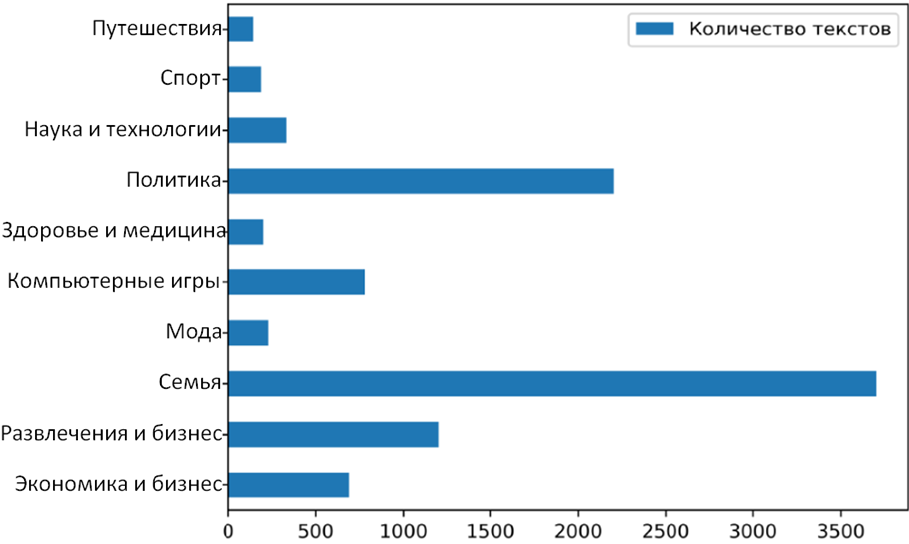
\includegraphics[width=0.75\columnwidth]{./img/ris14.png}
\centering
\caption{Диаграмма распределения по количеству, собранных текстов с сайтов}
\label{pic:ris14}
\end{figure}

\section{Разметка отобранных данных}

Для реализации моделей из третьего раздела, используются такие пакеты языка программирования python как: ufal.udpipe и wget. 
Как было сказано ранее для нахождения близости слов мы используем готовую модель, которую взяли с ресурса 
https://rusvectores.org/static/models с помощью пакета wget, принцип работы описан в \cite{neural08}. Данный пакет позволяет скачивать данные 
с веб ресурсов посредством GET запроса.

Для того чтобы модель word2vec, описанная в \cite{w2vec02} могла определить расстояние между словами, ей следует передать слово, ставится задача определить 
его часть речи, для того, чтобы автоматизировать такой процесс по определению части речи слова из текста, мы должны с помощью 
системы word2vec понять по слову какими категориями частей речи оно обладает, самые распространённые варианты – это 
существительные и глагол, далее после определения,  мы передаем их на анализ дистанции. 
Принцип работы модели представлен на (Рис. \ref{pic:ris15}):

\begin{figure}[H]
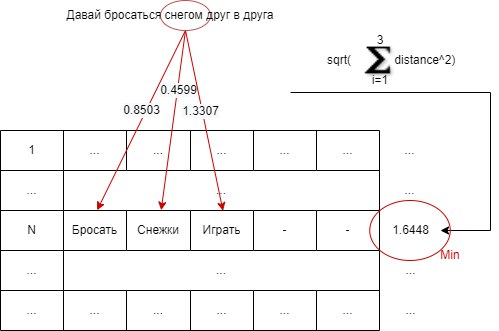
\includegraphics[width=0.75\columnwidth]{./img/ris15.png}
\centering
\caption{принцип работы word2vec}
\label{pic:ris15}
\end{figure}

В рамках данной работы используется модель ruwikiruscorpora\_tokens\_elmo\_1024\_2019 - модель UDPipe для нахождения синонимов. 
Данная модель позволяет узнать семантическую близость слов.

Чтобы начать применять указанную выше нейронную сеть непосредственно, следует подготовить действия виртуальных акторов так, 
чтобы ими могла оперировать частично или полностью сама нейронная сеть. Для этого возьмем разобьем описание каждого действия 
на ключевые слова так, что каждое действие будет ассоциировано с набором слов. При этом создан класс отражающий действие 
актора как сущность - VAAction(Virtual Actor Action), принцип которой описан в \cite{w2vec01}.

Данный класс содержит в себе описание действия и ключевые слова, описывающие данное действие. 
Среди таких слов отсутствуют предлоги, а сами слова представлены в нормальной форме 
(для существительных - именительный падеж единственное число).

Для построения сценариев берутся текста, полученные в разделе выше. Для каждого текста выделяются ключевые слова, 
которые наиболее близки к ключевым словам, описывающим действия акторов. Что происходит в процессе итерации через 
все слова текста так, что для каждого слова применяется считается значение близости слова к действию виртуального 
актора. Для работы с текстом создан класс WText (Web Text), который является ответственным за итерацию через все 
слова текста. С помощью методов класса задается функция, которая будет применяться к каждому слову. В качестве 
такой функции берется функция, которая находит близость слова с ключевыми словами экземпляра класса VAAction.

Также класс WText формирует набор определяющих текст слов, эти слова выбираются так, что значение 
семантической близости больше, чем заданный заранее порог, данной работе порог равен 0.08. После 
того как все тексты были переведены в экземпляры класса WText, была произведена оценка кол-ва 
текстов с одинаковым кол-вом определяющих слов. Такое распределение приведено на (Рис. \ref{pic:ris16}):

\begin{figure}[H]
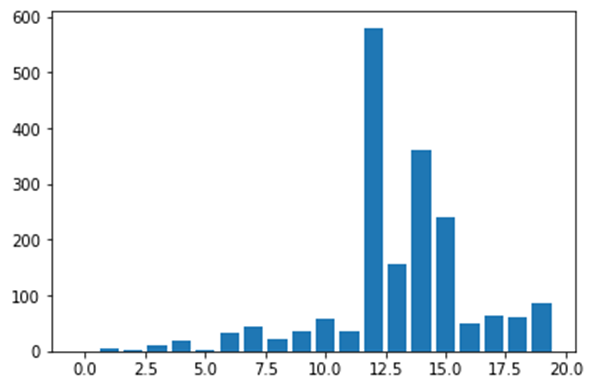
\includegraphics[width=0.75\columnwidth]{./img/ris16.png}
\centering
\caption{Распределение количества ключевых слов на текст}
\label{pic:ris16}
\end{figure}

Исходя из картинки видно, что подавляющее большинство текстов имеют более 10 определяющих слов. 
Каждому определяющему слову ставится в соответствие экземпляр класса VAAction, таким образом из 
текстов набираются сценарии из 10 последовательных действий.
Чтобы было удобнее формировать данные для обучения модели, определяющей поведение виртуальных акторов, 
реализуется метод получения последовательности состояний виртуальных агентов так, что переход в каждое последующее состояние.

\section{Реализация модели поведения виртуального актора}

По полученным размеченным данным на основании семантической близости слов выделенных и сопоставленных с заранее описанными действиями для акторов 
были получены следующие результаты. 
Суть первого эксперимента, состояла в предсказании 50 действий производимых  акторами, результаты эксперимента представлены на (Рис. \ref{pic:ris17}), (Рис. \ref{pic:ris18}):
\begin{figure}[H]
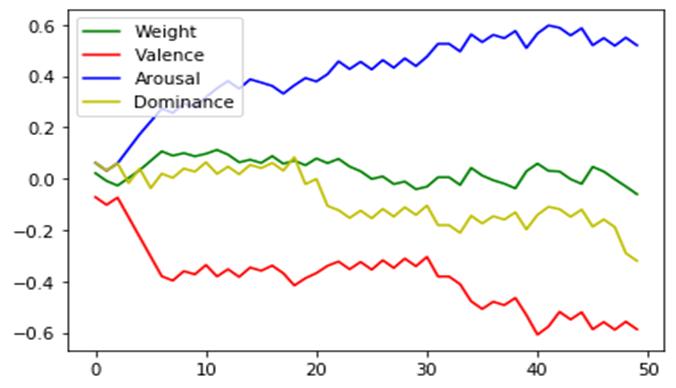
\includegraphics[width=0.75\columnwidth]{./img/ris17.png}
\centering
\caption{Оценки виртуального актора1}
\label{pic:ris17}
\end{figure}

\begin{figure}[H]
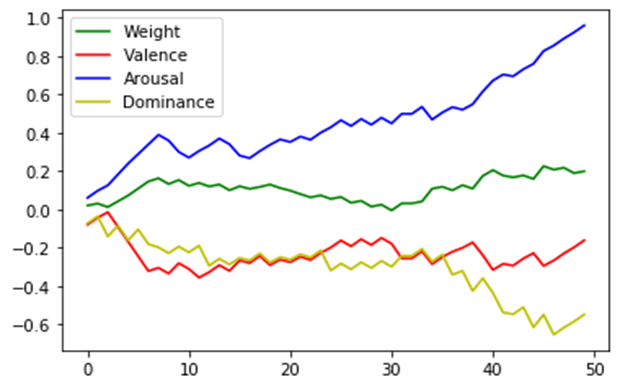
\includegraphics[width=0.75\columnwidth]{./img/ris18.png}
\centering
\caption{Оценки виртуального актора2}
\label{pic:ris18}
\end{figure}

В следующем эксперименте было проведено 10000 действий и была построена гистограмма распределения 
частоты действий выполняемых первым виртуальным актором., результаты представлены на (Рис. \ref{pic:ris19}):
\begin{figure}[H]
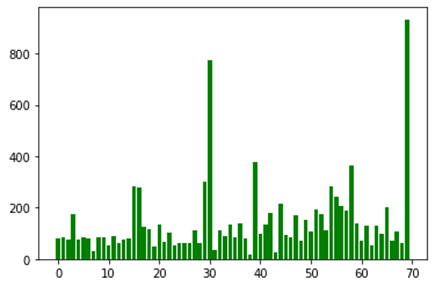
\includegraphics[width=0.75\columnwidth]{./img/ris19.png}
\centering
\caption{Частоты действий акторов}
\label{pic:ris19}
\end{figure}

\section{Выводы}

В данном разделе осуществляется описание реализации получения и разметки данных с ресурсов 
содержащих юмористические сюжеты. А так же последующим обучением модели, генерирующей 
поведение виртуального агента.

Была разработано программное обеспечение, позволяющее определять
семантическую принадлежность текста. А так же последующее определение 
семантической близости слов с заранее описанными действиями для виртуальных акторов. Группы 
действий которых впоследствии используются для обучения нейронной сети для 
последующей генерации юмористических сюжетов.
